\section{Evaluation}
\label{sec:evaluation}

In this Section, we present our experimental results.
First, we show the results about the randomness of the adopted random number generator.
Then, we show the results about the performance recorded by the simulation of the Cloud system.

% %
% EXPERIMENTAL ENVIRONMENT
% %
The experiments have been conducted on an Amazon EC2 c3.8xlarge instance, which is really indicated for high performance science and engineering applications\footnote{https://aws.amazon.com/ec2/instance-types/}.
The instance is equipped with 32 vCPU based on an Intel Xeon E5-2680 v2 (Ivy Bridge) processor, 30 GB of RAM and SSD with 900 IOPS.
It runs Debian 8.3 (Jessie), Python 3.5.2, and the Python-ported version of the official Leemis library for discrete-event simulation, indicated in \cite{leemis2006discrete}.
Our solution has been developed in Python, following the de-facto standard best-practices, stated in \cite{reitz2016,GooglePythonStyleguide}.

% %
% EXPERIMENTS: RANDOMNESS
% %
Let us now consider the results about the randomness of the adopted generator.
The randomness has been assessed by the following tests:

\begin{itemize}
	\item \textbf{Spectral Test:} this test is considered one of the most powerful tests to assess the quality of linear congruential generators \cite{knuth1981art}. It relies on the fact that the output of such generators form lines or hyperplanes when plotted on 2 or more dimensions. The less the distance between these lines or planes, the better the generator is. In fact, a smaller distance between lines or planes highlights a better uniform distribution.
	
	In Figure \ref{fig:experimental-analysis-randomness-spectral-16807,fig:experimental-analysis-randomness-spectral-48271,fig:experimental-analysis-randomness-spectral-58012} we show the test results for generators $(16807,2^{31}-1)$, $(48271,2^{31}-1)$ and $(58012,2^{31}-1)$, respectively.
	
	The results show that our generator $(58012,2^{31}-1)$ is much better than $(16807, 2^{31}-1)$, which was a past de-facto standard, and really similar to $(48271,2^{31}-1)$, which is the current de-facto standard, according to \cite{leemis2006discrete}.
	
	\item \textbf{Test of Extremes:} this test relies on the fact that if $U=U_{0},...,U_{d-1}$ is an iid sequence of Uniform(0,1) random variables, then $\max(U)^{d}$ is also a Uniform(0,1). The test leverages this property to measures, for every stream, how much the generated random values differ from the theoretical uniform distribution.
	
	The more the total number of fails is close to the expected value, i.e. $streams \cdot confidence$, the better the generator is.
	
	In Figure \ref{fig:experimental-analysis-randomness-extremes} we show the test results for the proposed generator $(508012,2^{31}-1, 256)$ with sample size $n=10000$, $k=1000$ bins, sequence size $d=5$ and $95\%$ level of confidence.
	%	
	The proposed generator shows critical values $v_{min}=913$ and $v_{max}=1088$ and 14 total fails (7 lower fails and 7 upper fails), that is not far from the theoretical accepted number of fails, i.e. $256*0.05=13$.
	The proposed generator successfully passed the test with a $94.531\%$ level of confidence.
	
	\item \textbf{Kolmogorov-Smirnov Analysis:} the test measures, at a certain confidence level, the biggest vertical distance between the theoretical cumulative distribution function and the empirical cumulative distribution function.
	The more the recorded distance $d$ is less than the critical value $d*$ for the considered level of confidence, the better the generator is.
	As the Kolmogorov-Smirnov analysis relies on pre-calculated randomness statistics, we have chosen to take into account the statistics obtained by the previous text of extremes.
	
	In Figure \ref{fig:experimental-analysis-randomness-kolmogorov-smirnov} we show the test results for the proposed generator $(508012,2^{31}-1, 256)$ with a $95\%$ level of confidence.
	%
	The proposed generator successfully passed the test, as $d=0.041<0.081=d*$.
	
\end{itemize}

\begin{figure}
  \label{fig:evaluation-randomness-spectral-16807}
  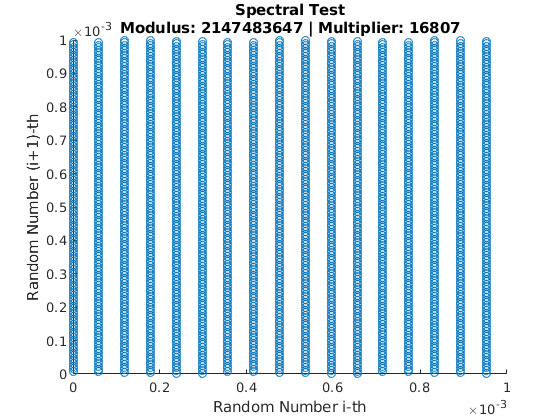
\includegraphics[width=\columnwidth]{fig/evaluation-randomness-spectral-16807}
  \caption{The Spectral Test to evaluate the randomness of the random number generator $(16807,2^{31}-1, 1)$ in the interval $(0, 10^{-3})$.}
\end{figure}

\begin{figure}
	\label{fig:evaluation-randomness-spectral-48271}
	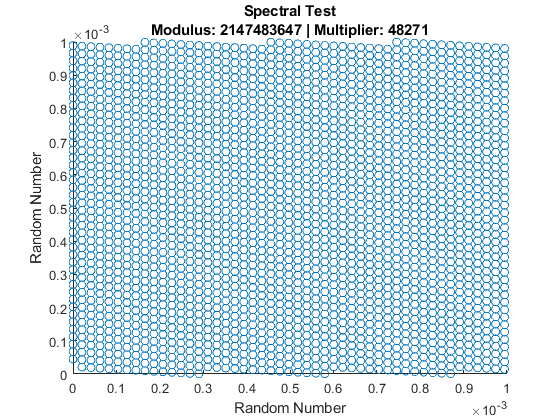
\includegraphics[width=\columnwidth]{fig/evaluation-randomness-spectral-48271}
	\caption{The Spectral Test to evaluate the randomness of the random number generator $(48271,2^{31}-1, 1)$ in the interval $(0, 10^{-3})$.}
\end{figure}

\begin{figure}
	\label{fig:evaluation-randomness-spectral-50812}
	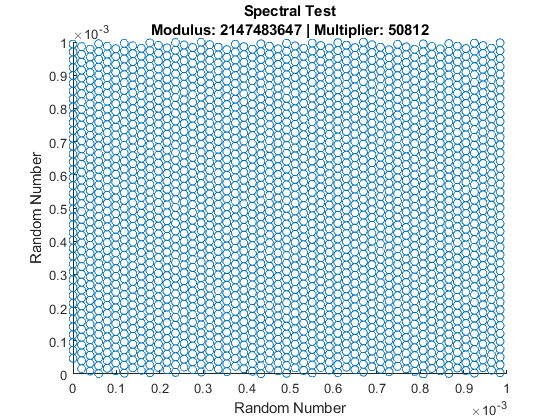
\includegraphics[width=\columnwidth]{fig/evaluation-randomness-spectral-50812}
	\caption{The Spectral Test to evaluate the randomness of the random number generator $(50812,2^{31}-1, 1)$ in the interval $(0, 10^{-3})$.}
\end{figure}

\begin{figure}
	\label{fig:evaluation-randomness-extremes-50812}
	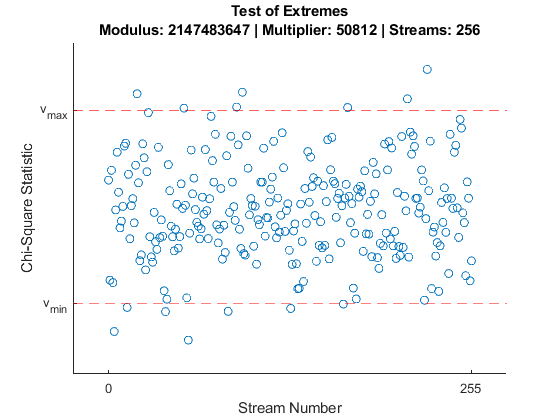
\includegraphics[width=\columnwidth]{fig/evaluation-randomness-extremes-50812}
	\caption{The Test of Extremes with $d=5$ to evaluate the randomness of the random number generator $(50812,2^{31}-1, 256)$.}
\end{figure}

\begin{figure}
	\label{fig:evaluation-randomness-kolmogorov-smirnov-50812}
	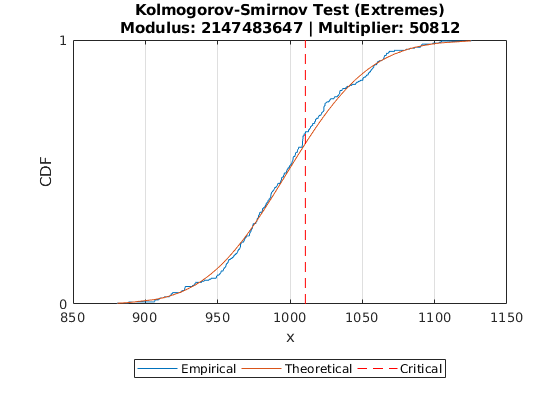
\includegraphics[width=\columnwidth]{fig/evaluation-randomness-kolmogorov-smirnov-50812}
	\caption{The Kolmogorov-Smirnov Analysis (leveraging the Test of Extremes with $d=5$) to evaluate the randomness of the random number generator $(50812,2^{31}-1, 256)$ with $0.95$ confidence level.}
\end{figure}


% %
% EXPERIMENTS: RESPONSE-TIME
% %
Let us now consider the results about the performance recorded by the simulation of the Cloud system.

\begin{figure}
  \label{fig:experimental-analysis-response-time}
  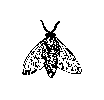
\includegraphics{fig/fly}
  \caption{Response Time Analysis.}
\end{figure}
